
\documentclass{report}

\usepackage[utf8]{inputenc}
\usepackage[italian]{babel}
\usepackage{import}
\usepackage{todonotes}
\usepackage{color}
\usepackage{rotating}
\usepackage[hidelinks]{hyperref}
\usepackage{url}
\usepackage{pdfpages}
\usepackage{siunitx}
\usepackage{pdflscape}
\usepackage{subfig}
\usepackage[euler]{textgreek}
\usepackage{mhchem}

\usepackage{multirow}

\usepackage{enumerate} 
\usepackage{amsmath}
\usepackage{amsfonts}

\usepackage[signatures,swapnames,sans]{frontespizio}

\usepackage{geometry}
\geometry{portrait, margin=3cm}
\usepackage{siunitx}
\usepackage{booktabs}

\renewcommand*\figurename{Figura}

\newcommand{\sub}[1]{\textsubscript{#1}}
\newcommand{\super}[1]{\textsuperscript{#1}}
\newcommand{\parallelsum}{\mathbin{\!/\mkern-5mu/\!}}

\newcommand{\Fig}[0]{Fig.}

\usepackage{titlesec}

\titleformat{\chapter}{\normalfont\huge}{}{20pt}{\huge\bfseries}

\linespread{1.3}


%% COMANDI UTILI
%\begin{table}[h]
%	\centering
%	\begin{tabular}{|c|c|c|}
%	\cline{2-3} 
%	\multicolumn{1}{c|}{} & \textbf{Valore nominale} & \textbf{Valore misurato}\\ 
%		%\hline
%		%{} & \textbf{Valore nominale} & \textbf{Valore misurato} \\ 
%		\hline
%		$\mathbf{R_1}$ & \SI{18}{k\ohm} & \SI{17.977}{k\ohm} \\ 
%		\hline
%		$\mathbf{R_2}$& \SI{1.8}{k\ohm} & \SI{1.815}{k\ohm} \\ 
%		\hline
%	\end{tabular}
%\caption{Misure delle resistenze utilizzate per il circuito.}
%\label{table:mis_res}
%\end{table}
%\begin{figure}[h!]
%\centering
%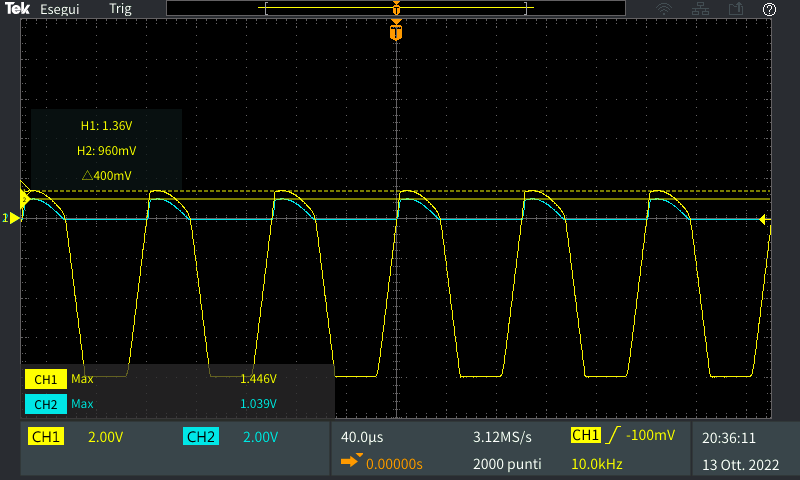
\includegraphics[height=6.5cm]{immagini/TEK00018}\\(a)\\[1ex]
%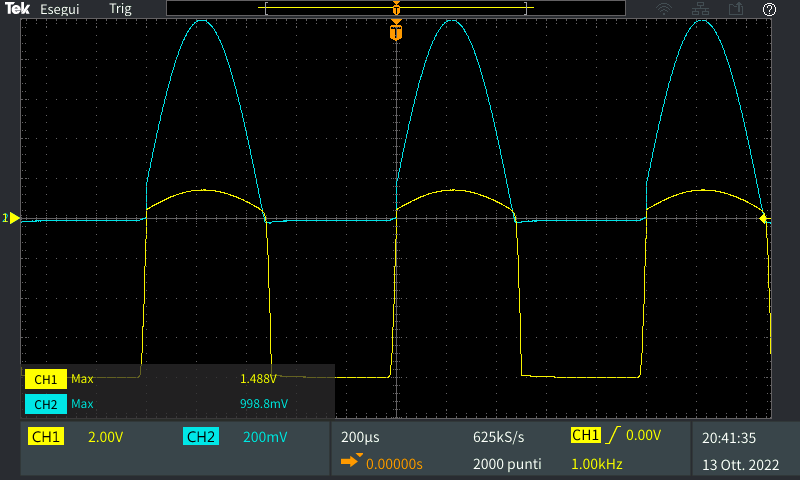
\includegraphics[height=6.5cm]{immagini/TEK00019}\\(b)
%\caption{Risposta del circuito con accoppiamento DC (a) e accoppiamento AC (b).}
%	\label{figura:accopp}
%\end{figure}

\begin{document}
\addtocounter{chapter}{+1}
	\begin{frontespizio}
		\Margini{3cm}{3cm}{3cm}{3cm}
		\Universita{Bergamo}
		\Logo[43.332mm]{unibg-mark}
		\Divisione{Scuola di Ingegneria}
		\Corso[Laurea Magistrale]{Ingegneria Informatica}
		\Titolo{Laboratorio di Elettronica}
		\Sottotitolo{Relazione esperienza di laboratorio 2}
		\Punteggiatura{}
		\NRelatore{Prof.}{Prof.}
		\Relatore{Luigi Gaioni}
		\Candidato[1058231]{Giulia Allievi}
		\Candidato[1059640]{Martina Fanton}
		\Annoaccademico{2022--2023}
		\begin{Preambolo*}
			\usepackage[italian]{babel}
			\usepackage[T1]{fontenc}
			\usepackage[utf8]{inputenc}
			\usepackage{microtype}
			\usepackage{lmodern}
			\graphicspath{{img/}}
			
			\renewcommand{\frontinstitutionfont}{\fontsize{14}{17}\bfseries\scshape}
			\renewcommand{\fronttitlefont}{\fontsize{17}{21}\bfseries\scshape}
			\renewcommand{\frontfootfont}{\fontsize{12}{14}\bfseries\scshape}
		\end{Preambolo*}
	\end{frontespizio}

%----------------------------------------------------------------------------------------
%	PAGINA BIANCA
%----------------------------------------------------------------------------------------
\newpage
\null
\thispagestyle{empty}
\newpage

%----------------------------------------------------------------------------------------
%	INTRO
%----------------------------------------------------------------------------------------
% Ho cambiato la struttura per questa relazione così rimane tutto nominato con il numero 2
\chapter{Relazione attività di laboratorio 2}
\section*{Introduzione}
Nei circuiti realizzati in questa attività di laboratorio utilizzeremo dei diodi, in particolare i diodi 1N4148. Un diodo è un dispositivo non lineare perché la corrente che fluisce al suo interno ha un andamento esponenziale in funzione della tensione applicata ai suoi capi, inoltre non è simmetrico perché la corrente può fluire in un solo verso, ovvero dall'anodo al catodo, e non viceversa.
\begin{figure}[h]
	\centering
	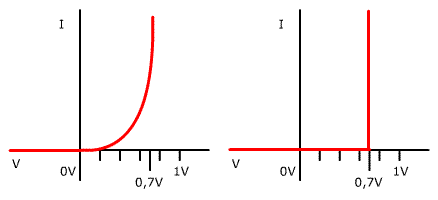
\includegraphics[height=5cm]{immagini/diodo}
	\caption{Caratteristica reale (a destra) e ideale (a destra) di un diodo.}
	\label{figura:diodo}
\end{figure}
\\Nella figura precedente, la figura \ref{figura:diodo} si possono vedere la caratteristica reale ed ideale di un diodo: per studiare più facilmente i circuiti si approssima il comportamento di un diodo e lo si considera spento (OFF) se la tensione applicata ai suoi capi è minore di \SI{0.7}{\volt}; al contrario, se la tensione ai suoi capi è maggiore di questo valore, il diodo è acceso (ON) e lascia fluire la corrente dall'anodo al catodo con una caduta di tensione ai suoi capi di \SI{0.7}{\volt}.
\newpage
\section{Circuito 1: raddrizzatore passivo a semionda}
\subsection{Schema del circuito e Funzione di Trasferimento}Il primo circuito è il raddrizzatore più semplice che si può realizzare. \`E costituito da un diodo e da una resistenza, il segnale viene applicato all'anodo del diodo e l'uscita del circuito è prelevata al catodo del diodo. Il circuito non viene alimentato, perciò abbiamo un raddrizzatore passivo. \par
\begin{figure}[h]
	\centering
	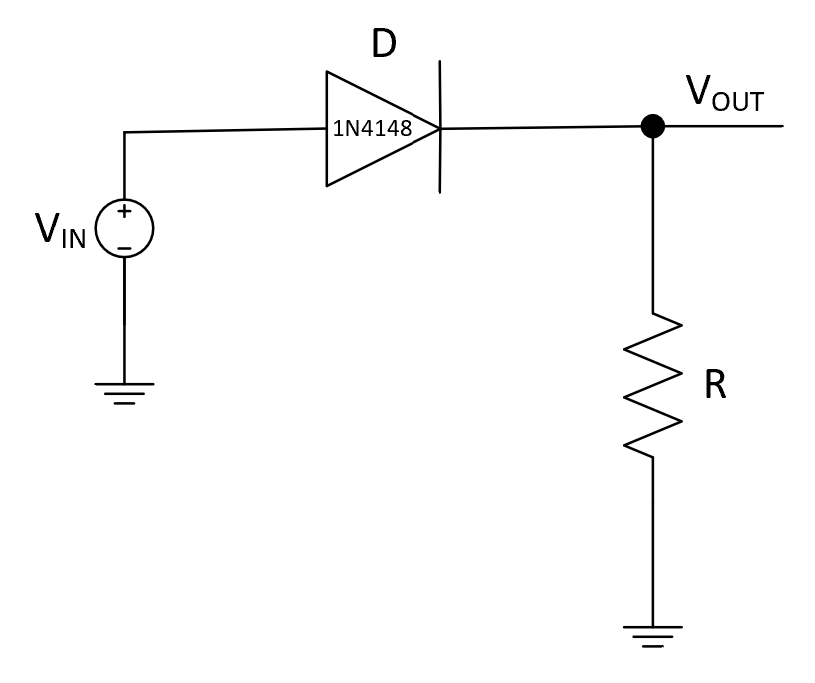
\includegraphics[height=6.5cm]{immagini/schema1}
	\caption{Schema del raddrizzatore passivo a semionda.}
	\label{figura:schema1}
\end{figure}
\noindent La funzione di trasferimento di questo raddrizzatore è:
\begin{equation}
   \begin{cases}
   V_{in}< \SI{0.7}{\volt}\;\;\rightarrow \mathrm{D\;OFF} \Rightarrow V_{out} =\SI{0}{\volt}\\
   V_{in}\ge \SI{0.7}{\volt}\;\;\rightarrow \mathrm{D\;ON}\;\; \Rightarrow V_{out} = V_{in}-\SI{0.7}{\volt}
   \end{cases}
\end{equation}
\subsection{Analisi e dati sperimentali}
Prima di realizzare il circuito, misuriamo con il multimetro la caduta di tensione ai capi del diodo, contattando l'anodo con la sonda rossa (+) e il catodo con quella nera (-). Dato che questo componente non è simmetrico, il catodo è segnalato da una fascia di colore nero. La caduta di tensione misurata è \SI{0.612}{\volt}, infatti la caduta di tensione di una giunzione p-n è solitamente compresa fra \SI{0.6}{\volt} e \SI{0.7}{\volt}. \par
Il raddrizzatore passivo a semionda realizzato in laboratorio è mostrato in figura \ref{figura:circuito1}. Il nostro obiettivo è quello di studiare il suo comportamento al variare della frequenza della sinusoide in ingresso ed al variare della tensione ai capi del diodo. Per fare variare quest'ultimo parametro, utilizzeremo 4 resistenze di diverso valore, i valori nominali e misurati sono stati riportati in tabella \ref{table:misure1}. \par
\begin{figure}[h!]
	\centering
	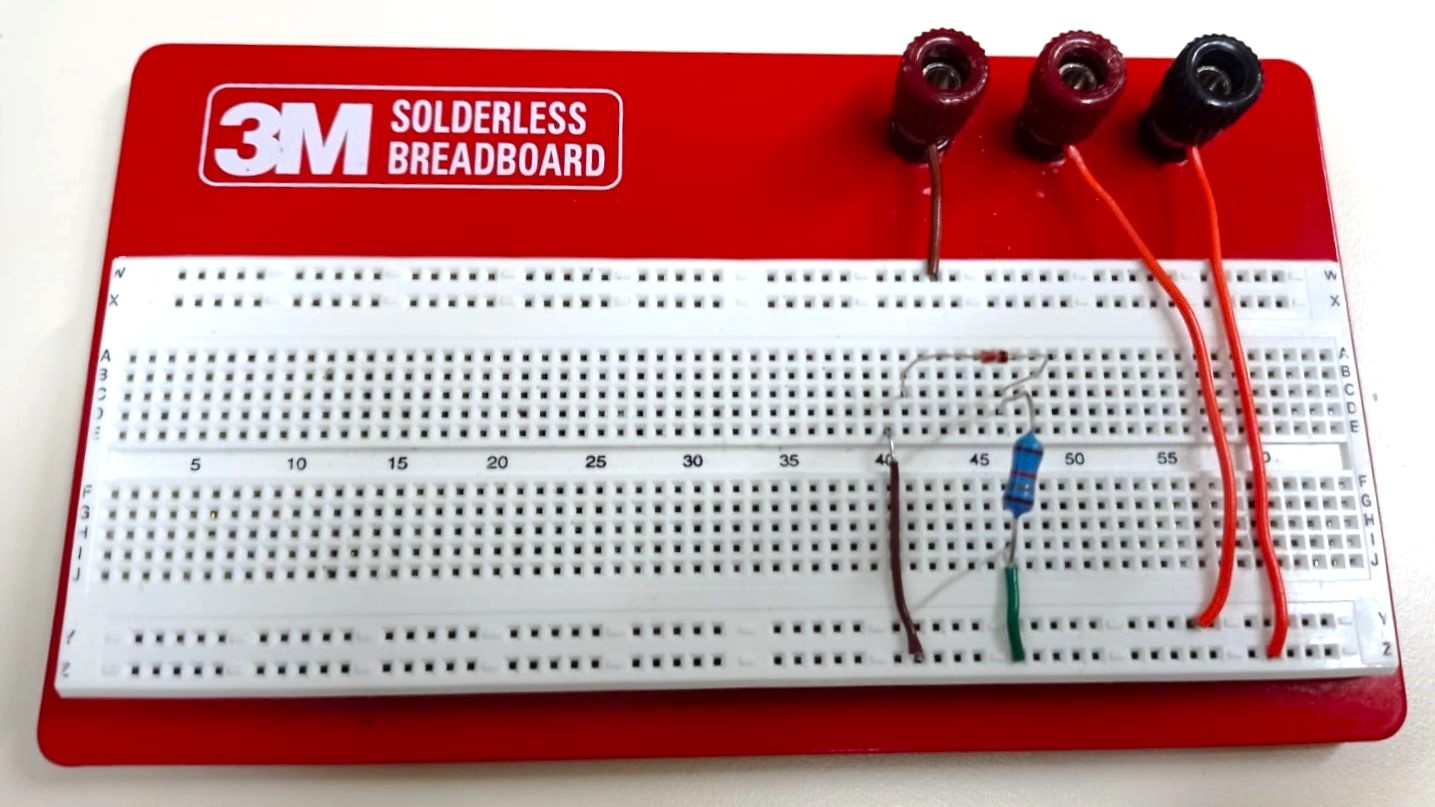
\includegraphics[height=6.5cm]{immagini/circuito1}
	\caption{Fotografia del raddrizzatore passivo a semionda realizzato in laboratorio con $\displaystyle\mathrm{R=\SI{18}{k\ohm}}$.}
	\label{figura:circuito1}
\end{figure}
\begin{table}[h!]
	\centering
	\begin{tabular}{|c|c|c|}
		\cline{2-3} 
		\multicolumn{1}{c|}{} & \textbf{Valore nominale} & \textbf{Valore misurato}\\ 
		\hline
		$\mathbf{R_1}$ & \SI{18}{k\ohm} & \SI{17.977}{k\ohm} \\ 
		\hline
		$\mathbf{R_2}$ & \SI{33}{k\ohm} & \SI{37.630}{k\ohm} \\ 
		\hline
		$\mathbf{R_3}$ & \SI{56}{k\ohm} & \SI{54.742}{k\ohm} \\ 
		\hline
		$\mathbf{R_4}$ & $\displaystyle\mathrm{\SI{82}{k\ohm}+\SI{18}{k\ohm}=\SI{100}{k\ohm}}$ & $\displaystyle\mathrm{\SI{80.717}{k\ohm+}\SI{17.977}{k\ohm}=\SI{98.694}{k\ohm}}$ \\ 
		\hline
	\end{tabular}
	\caption{Misure delle resistenze utilizzate nel raddrizzatore a semionda passivo.}
	\label{table:misure1}
\end{table}
Facciamo variare la frequenza della sinusoide in ingresso da \SI{1}{k\hertz} a \SI{1}{M\hertz} prendendo un punto per ogni decade e misuriamo con l'oscilloscopio l'ampiezza del segnale in ingresso e del segnale in uscita, quindi ne facciamo la differenza. Ripetiamo queste misure per i quattro valori di resistenza, i valori ricavati sono riportati in tabella \ref{table:misTensioni1}.
\begin{table}[h!]
	\centering
	\begin{tabular}{|c|c|c|c|c|c|}
		\cline{2-5} 
		\multicolumn{1}{c|}{} & \textbf{1 kHz} &  \textbf{10 kHz}  &  \textbf{100 kHz}  &  \textbf{1 MHz}  &\multicolumn{1}{c}{} \\ 
		\hline
		\multirow{3}{*}{\textbf{18 k\textOmega}} & \SI{980}{m\volt} & \SI{980}{m\volt} & \SI{980}{m\volt} & \SI{980}{m\volt} & $\mathbf{V_{in}}$ \\
		\cline{2-6}
		& \SI{520}{m\volt} & \SI{540}{m\volt} & \SI{540}{m\volt} & \SI{540}{m\volt} & $\mathbf{V_{out}}$\\
		\cline{2-6}
		& \SI{460}{m\volt} & \SI{440}{m\volt} & \SI{440}{m\volt} & \SI{440}{m\volt} & $\mathbf{V_D}$\\
		\hline
		\multirow{3}{*}{\textbf{33 k\textOmega}} & \SI{980}{m\volt} & \SI{980}{m\volt} & \SI{980}{m\volt} & \SI{980}{m\volt} & $\mathbf{V_{in}}$ \\
		\cline{2-6}
		& \SI{560}{m\volt} & \SI{580}{m\volt} & \SI{560}{m\volt} & \SI{540}{m\volt} & $\mathbf{V_{out}}$\\
		\cline{2-6}
		& \SI{420}{m\volt} & \SI{400}{m\volt} & \SI{420}{m\volt} & \SI{440}{m\volt} & $\mathbf{V_D}$\\
		\hline
		\multirow{3}{*}{\textbf{56 k\textOmega}} & \SI{960}{m\volt} & \SI{980}{m\volt} & \SI{980}{m\volt} & \SI{980}{m\volt} & $\mathbf{V_{in}}$ \\
		\cline{2-6}
		& \SI{580}{m\volt} & \SI{580}{m\volt} & \SI{580}{m\volt} & \SI{540}{m\volt} & $\mathbf{V_{out}}$\\
		\cline{2-6}
		& \SI{380}{m\volt} & \SI{400}{m\volt} & \SI{400}{m\volt} & \SI{440}{m\volt} & $\mathbf{V_D}$\\
		\hline
		\multirow{3}{*}{\textbf{100 k\textOmega}} & \SI{960}{m\volt} & \SI{980}{m\volt} & \SI{980}{m\volt} & \SI{980}{m\volt} & $\mathbf{V_{in}}$ \\
		\cline{2-6}
		& \SI{620}{m\volt} & \SI{620}{m\volt} & \SI{600}{m\volt} & \SI{560}{m\volt} & $\mathbf{V_{out}}$\\
		\cline{2-6}
		& \SI{340}{m\volt} & \SI{360}{m\volt} & \SI{380}{m\volt} & \SI{420}{m\volt} & $\mathbf{V_D}$\\
		\hline
	\end{tabular}
	\caption{Misure delle tensioni al variare della frequenza e della tensione ai capi del diodo.}
	\label{table:misTensioni1}
\end{table}
\\Dalla tabella precedente, vediamo che la caduta di tensione ai capi del diodo aumenta al diminuire della resistenza, perciò $\mathrm{V_D}$ aumenta all'aumentare della corrente che scorre nel diodo. In figura \ref{figura:res} è riportato il grafico della tensione in ingresso ed in uscita al circuito quando si utilizza la resistenza da \SI{18}{k\ohm} e quando si utilizza invece quella da \SI{100}{k\ohm}.\par
\begin{figure}[h!]
\centering
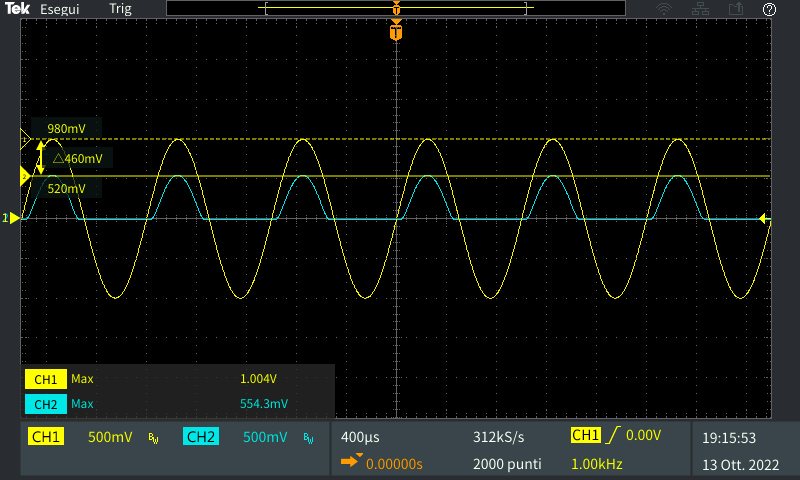
\includegraphics[height=4.6cm]{immagini/TEK00000}
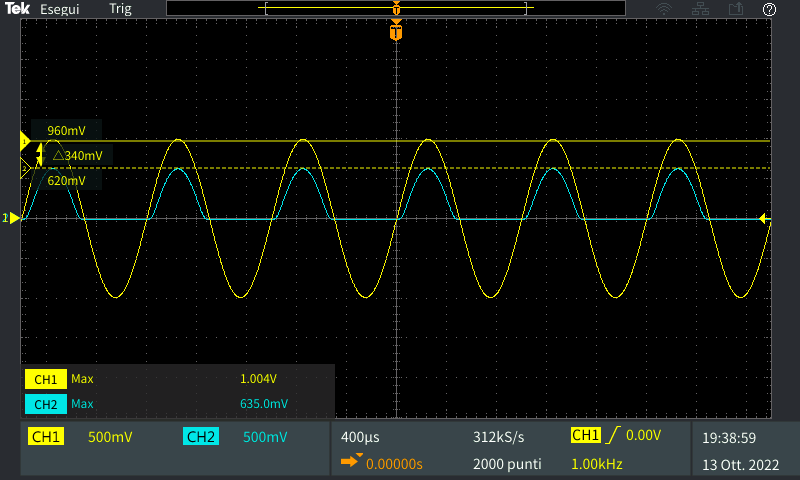
\includegraphics[height=4.6cm]{immagini/TEK00003}
\caption{Risposta del circuito con $\mathrm{R=18k\Omega}$ (sinistra) e con $\mathrm{R=100k\Omega}$ (destra).}
	\label{figura:res}
\end{figure}
\noindent La tensione ai capi del diodo è anche proporzionale alla frequenza, infatti $\mathrm{V_D}$ aumenta all'aumentare della frequenza. Nella figura successiva (figura \ref{figura:freq}) è mostrata la risposta del circuito a due sinusoidi, una di frequenza \SI{1}{k\hertz} e l'altra di frequenza \SI{1}{M\hertz}, con resistenza di \SI{18}{k\ohm}.
\begin{figure}[h!]
\centering
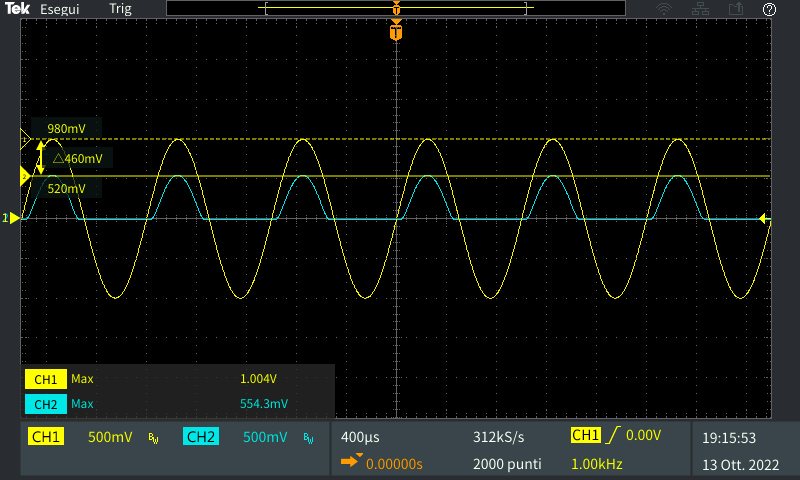
\includegraphics[height=4.6cm]{immagini/TEK00000}
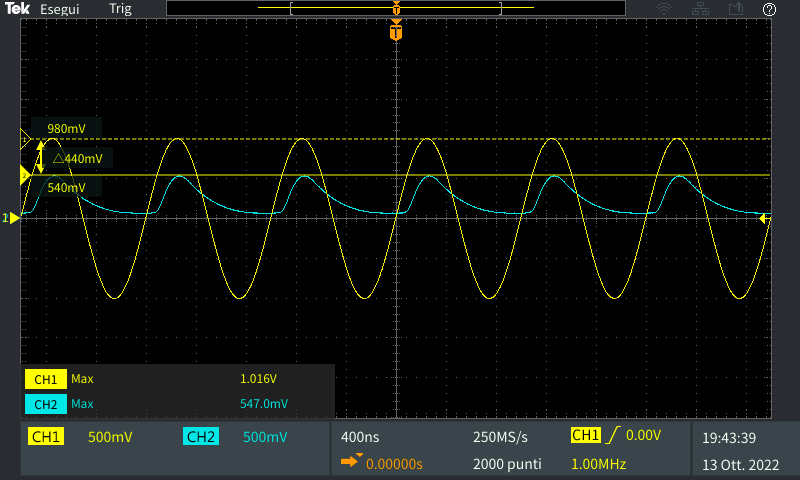
\includegraphics[height=4.6cm]{immagini/TEK00007}
\caption{Risposta del circuito con $\mathrm{f=\SI{1}{k\hertz}}$ (sinistra) e con $\mathrm{f=\SI{1}{M\hertz}}$ (destra).}
	\label{figura:freq}
\end{figure}
\\Dai grafici precedenti vediamo che il circuito raddrizza solo le semionde positive, mentre quelle negative vengono azzerate, proprio come ci aspettiamo dalla teoria. \par
Dalla figura \ref{figura:freq} a destra possiamo vedere che ad alte frequenza il segnale viene distorto, questo è ancor più visibile per valori crescenti di R. La distorsione è dovuta al fatto che le velocità di accensione e spegnimento del diodo sono finite: quando il diodo passa alla fase di OFF, impiega un certo tempo per spegnersi e ad alte frequenze il tempo di spegnimento è confrontabile con il periodo della sinusoide in ingresso, perciò se inizia un nuovo periodo senza che il diodo si sia completamente spento, il segnale viene sia ritardato che distorto, quindi l'uscita non è più una semionda. Il primo quarto di sinusoide resta corretto perché il tempo di accensione del diodo è più piccolo del tempo di spegnimento e non influenza quindi le prestazioni del raddrizzatore. \par
Per spiegare questa perdita di prestazioni nel secondo tratto di semionda bisogna considerare che ad alta frequenza il diodo si comporta come una capacità, che va a scaricarsi sulla resistenza R. L'andamento delle tensioni e delle correnti non seguirà più le formule del diodo, ma quelle di un circuito RC, perciò l'andamento della tensione nel tempo segue le leggi di un condensatore che si scarica su una resistenza.\par
Se la resistenza ha un valore elevato, non favorisce la scarica del condensatore, quindi la distorsione del segnale in uscita al raddrizzatore è maggiore. Nella figura successiva, la figura \ref{figura:caso1}, è riportato il grafico della tensione in uscita al circuito quando la resistenza vale \SI{100}{k\ohm} e la frequenza della sinusoide in ingresso è \SI{1}{M\hertz}, vediamo che il comportamento del circuito non è più quello di un raddrizzatore. \par
\begin{figure}[h!]
	\centering
	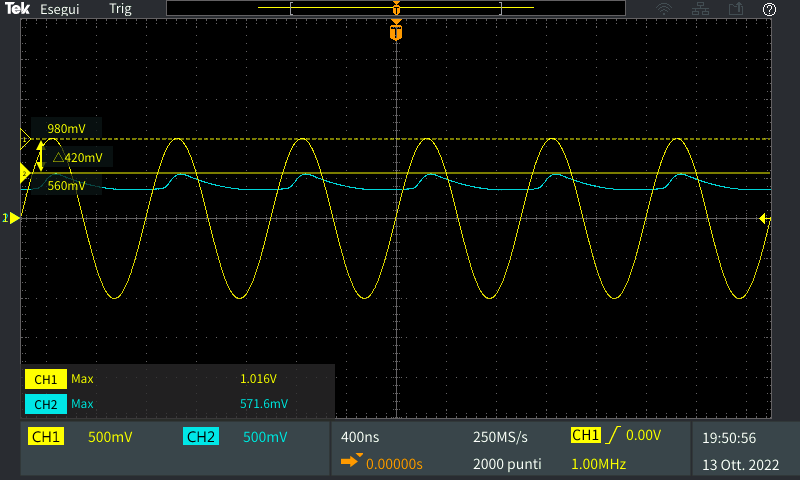
\includegraphics[height=6.5cm]{immagini/TEK00015}
	\caption{Comportamento distorto del circuito.}
	\label{figura:caso1}
\end{figure} 
\noindent Per frequenze e resistenze intermedie le prestazioni non sono così degradate, la tensione in uscita è solo leggermente distorta nella parte decrescente della semionda. In figura \ref{figura:caso2} è riportata la risposta del circuito ad una sinusoide di frequenza \SI{100}{k\hertz} con la resistenza da \SI{33}{k\ohm}.
\begin{figure}[h!]
	\centering
	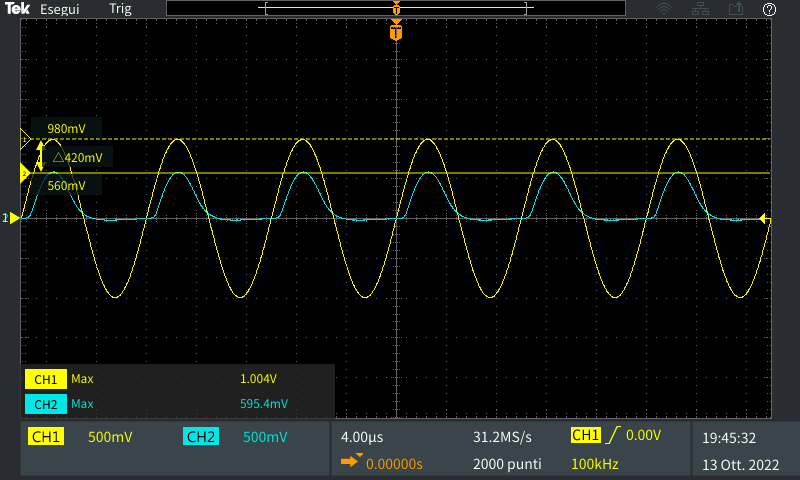
\includegraphics[height=6cm]{immagini/TEK00008}
	\caption{Risposta del circuito ad una sinusoide di frequenza \SI{100}{k\hertz} e resistenza da \SI{33}{k\ohm}.}
	\label{figura:caso2}
\end{figure} 
\newpage
\section{Circuito 2: raddrizzatore a semionda di precisione}
\subsection{Schema del circuito e Funzione di Trasferimento}
Modifichiamo il circuito di prima introducendo un amplificatore operazionale, il \textmu A741. Il diodo si trova ora in reazione all'amplificatore operazionale, nella cosiddetta configurazione a superdiodo: con queste connessioni otteniamo un raddrizzatore di precisione perché eliminiamo la caduta di tensione della giunzione p-n del diodo. Lo svantaggio è che l'OPAMP è un dispositivo attivo, quindi dovremo alimentare il circuito.\par
\begin{figure}[h!]
	\centering
	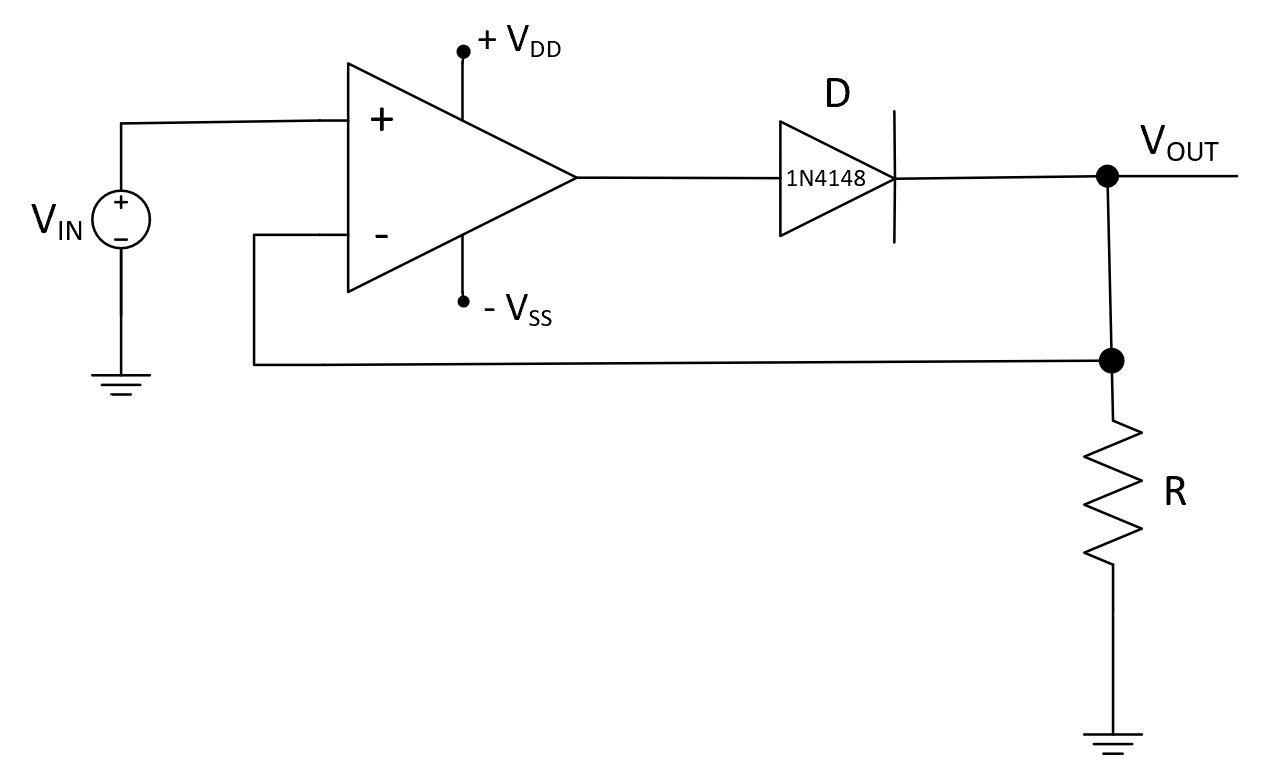
\includegraphics[height=7.5cm]{immagini/schema2}
	\caption{Schema del raddrizzatore a semionda di precisione.}
	\label{figura:schema2}
\end{figure}
\noindent La funzione di trasferimento è:
\begin{equation}
   \begin{cases}
   V_{in}\le \SI{0}{\volt}\;\;\rightarrow \mathrm{D\;OFF} \Rightarrow V_{out} =\SI{0}{\volt}\\
   V_{in}> \SI{0}{\volt}\;\;\rightarrow \mathrm{D\;ON}\;\; \Rightarrow V_{out} = V_{in}
   \end{cases}
\end{equation}
\subsection{Analisi e dati sperimentali}
Montiamo il circuito sulla breadbord e la alimentiamo. Impostiamo la tensione positiva a +\SI{10}{\volt} e la tensione negativa a \SI{-10}{\volt}. Il circuito realizzato è mostrato in figura \ref{figura:circ2}. \par
\begin{figure}[h!]
	\centering
	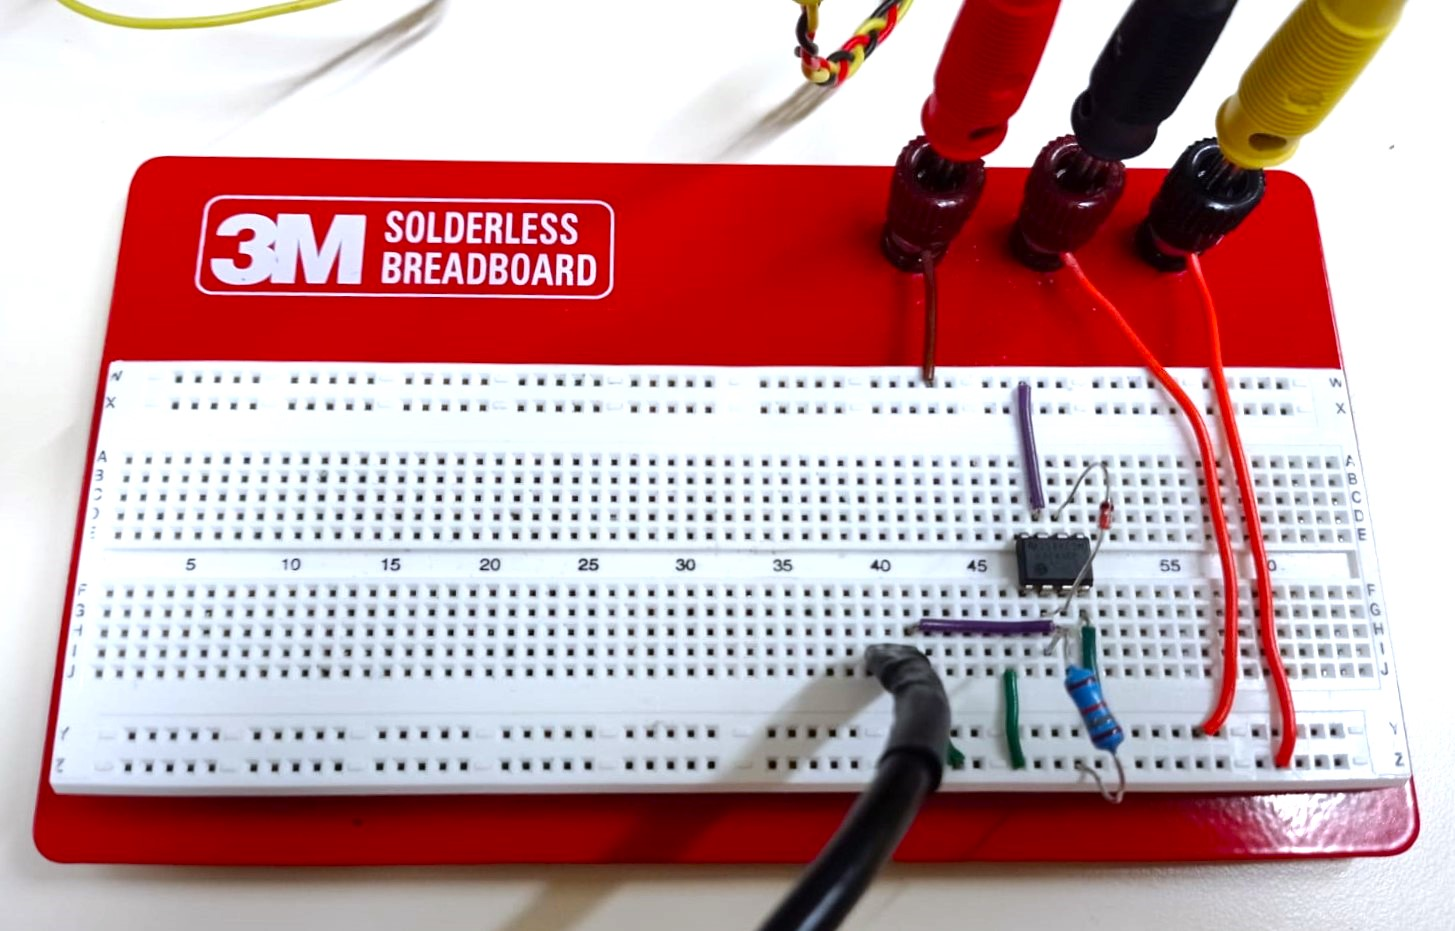
\includegraphics[height=7cm]{immagini/circuito2}
	\caption{Fotografia del raddrizzatore a semionda di precisione realizzato in laboratorio.}
	\label{figura:circ2}
\end{figure}
Fissiamo la resistenza a \SI{18}{k\ohm} e studiamo la risposta del circuito a due sinusoidi, una di frequenza \SI{1}{k\hertz} e l'altra di frequenza \SI{10}{k\hertz}. Di seguito, in figura \ref{figura:1khz}, si riporta il grafico della risposta del circuito alla prima sinusoide, mentre nella figura \ref{figura:10khz} la risposta alla seconda sinusoide. \par
Con l'oscilloscopio, andiamo a misurare la tensione massima dei nodi $\mathrm{V_1}$ e $\mathrm{V_{out}}$ e ne facciamo la differenza, le misure sono riportate in tabella \ref{table:mis2}.
\begin{figure}[h!]
\centering
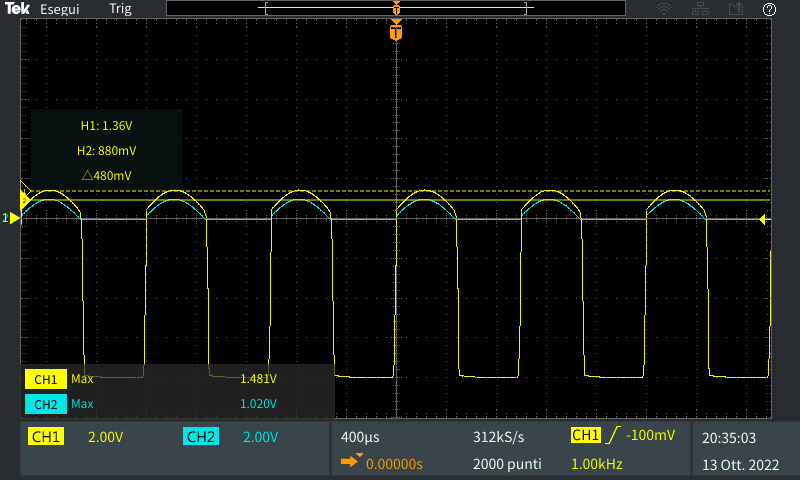
\includegraphics[height=4.6cm]{immagini/TEK00017}
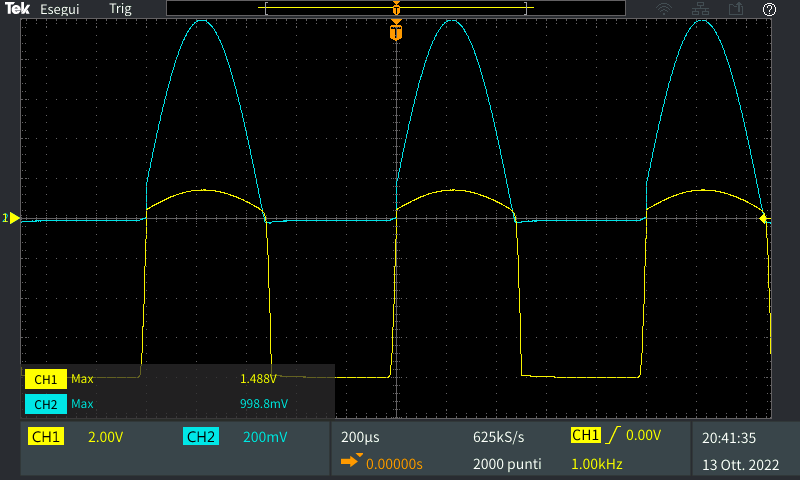
\includegraphics[height=4.6cm]{immagini/TEK00019}
\caption{Risposta del circuito in scala (sinistra) e non in scala (destra) con $\mathrm{f= \SI{1}{k\hertz}}$.}
	\label{figura:1khz}
\end{figure}\begin{figure}[h!]
\centering
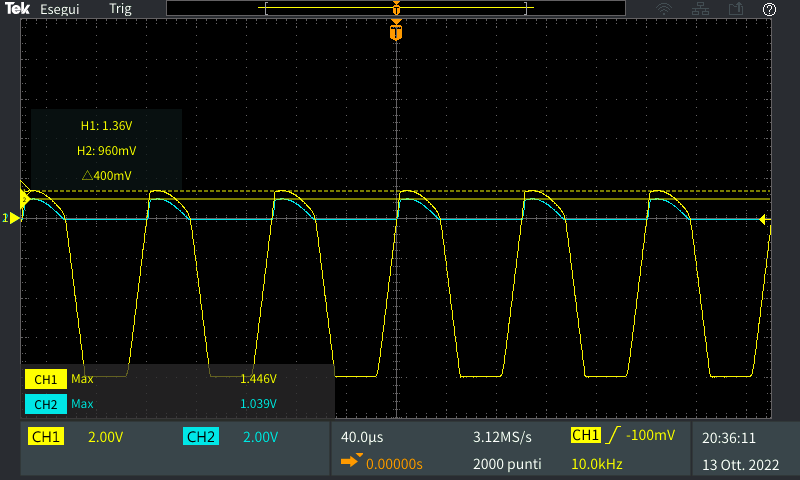
\includegraphics[height=4.6cm]{immagini/TEK00018}
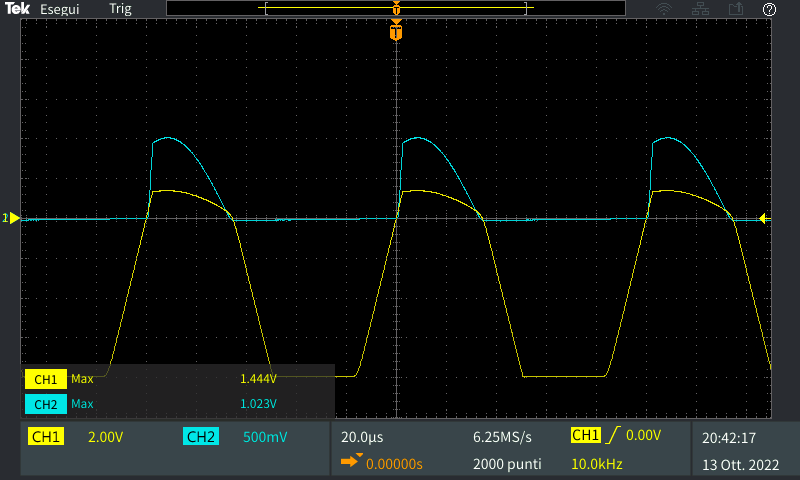
\includegraphics[height=4.6cm]{immagini/TEK00020}
\caption{Risposta del circuito in scala (sinistra) e non in scala (destra) con $\mathrm{f= \SI{10}{k\hertz}}$.}
	\label{figura:10khz}
\end{figure}
\begin{table}[h!]
	\centering
	\begin{tabular}{|c|c|c|c|}
		\cline{2-3} 
		\multicolumn{1}{c|}{} & \textbf{1 kHz} &  \textbf{10 kHz}  &\multicolumn{1}{c}{} \\ 
		\hline
		\multirow{3}{*}{\textbf{18 k\textOmega}} &  \SI{1.36}{\volt} & \SI{1.36}{\volt} & $\mathbf{V_{1}}$ \\
		\cline{2-4}
		& \SI{880}{m\volt} & \SI{960}{m\volt} & $\mathbf{V_{out}}$\\
		\cline{2-4}
		& \SI{480}{m\volt}  & \SI{400}{m\volt} & $\mathbf{V_D}$\\
		\hline
	\end{tabular}
	\caption{Misure delle tensioni al variare della frequenza.}
	\label{table:mis2}
\end{table}
\\\\\\\\\\Come ci aspettiamo, quando il diodo è ON l'amplificatore si trova nella configurazione a buffer, perciò la tensione del nodo in uscita è pari alla tensione del nodo in ingresso, mentre il nodo $\mathrm{V_1}$ segue il nodo $\mathrm{V_{out}}$ ma è traslato di circa +\SI{0.7}{\volt} per la caduta di tensione ai capi del diodo. Quando la tensione in ingresso è negativa, il diodo è OFF e l'ingresso invertente è collegato a massa tramite la resistenza. Dato che le correnti in ingresso all'operazionale sono trascurabili, sulla resistenza non c'è caduta di tensione e sia l'ingresso invertente che il nodo $\mathrm{V_{out}}$ si trovano a massa. L'OPAMP non è in reazione, ma in anello aperto, quindi si comporta come un comparatore. Visto che l'ingresso non invertente si trova ad una tensione negativa mentre quello invertente a massa, la tensione satura all'alimentazione negativa, perciò vale \SI{-10}{\volt}.\par
Se analizziamo la risposta alla prima sinusoide, vediamo che il circuito si comporta correttamente, come descritto nel paragrafo precedente. Per la seconda sinusoide invece, il comportamento è diverso da quello teorico perché le semionde non sono raddrizzate correttamente. Il degradamento delle prestazioni è dovuto ad una non-idealità dell'amplificatore operazionale, lo slew rate. Un OPAMP reale non è in grado di passare istantaneamente da una tensione di \SI{0}{\volt} all'alimentazione negativa, ma per erogarla impiegherà un certo intervallo di tempo per giungere a questo valore. Lo slew rate è definito come la pendenza della retta che descrive questa transizione e si misura in $[V/\mu s]$. Dal grafico precedente ricaviamo uno slew rate di [??], a fronte di un valore teorico (presente nel datasheet) di [??]. \par
Il raddrizzatore realizzato è detto di precisione perché si riesce a ``cancellare'' dal segnale in uscita l'offset dovuto alla caduta di tensione ai capi del diodo, tuttavia non è adatto per applicazioni ad alte frequenze a causa delle limitazioni operative dell'OPAMP. 
\newpage
\section{Circuito 3: raddrizzatore a doppia semionda}
\subsection{Schema del circuito e Funzione di Trasferimento}
In questo circuito (come mostrato nella figura \ref{figura:schema3}), a differenza dei precedenti due, sono presenti due diodi: il primo è collegato con l'anodo all'uscita dell'OPAMP e con il catodo al noto $\displaystyle\mathrm{V_{out}}$, mentre il secondo è posizionato nella retroazione del circuito, con l'anodo collegato al nodo $\displaystyle\mathrm{V_{in}}$ e il catodo a $\displaystyle\mathrm{V_{out}}$.\par
La differenza principale di questo circuito rispetto ai precedenti è che non raddrizza solo le semionde negative o positive, ma entrambe, per questo il raddrizzatore è detto \textit{a doppia semionda}. \par
Inoltre il raddrizzatore a doppia semionda presenta due retroazioni negative e in particolare quella costituita dalla sola resistenza R è sempre chiusa permettendo al circuito in esame di non operare in anello aperto.\par
\begin{figure}[h]
	\centering
	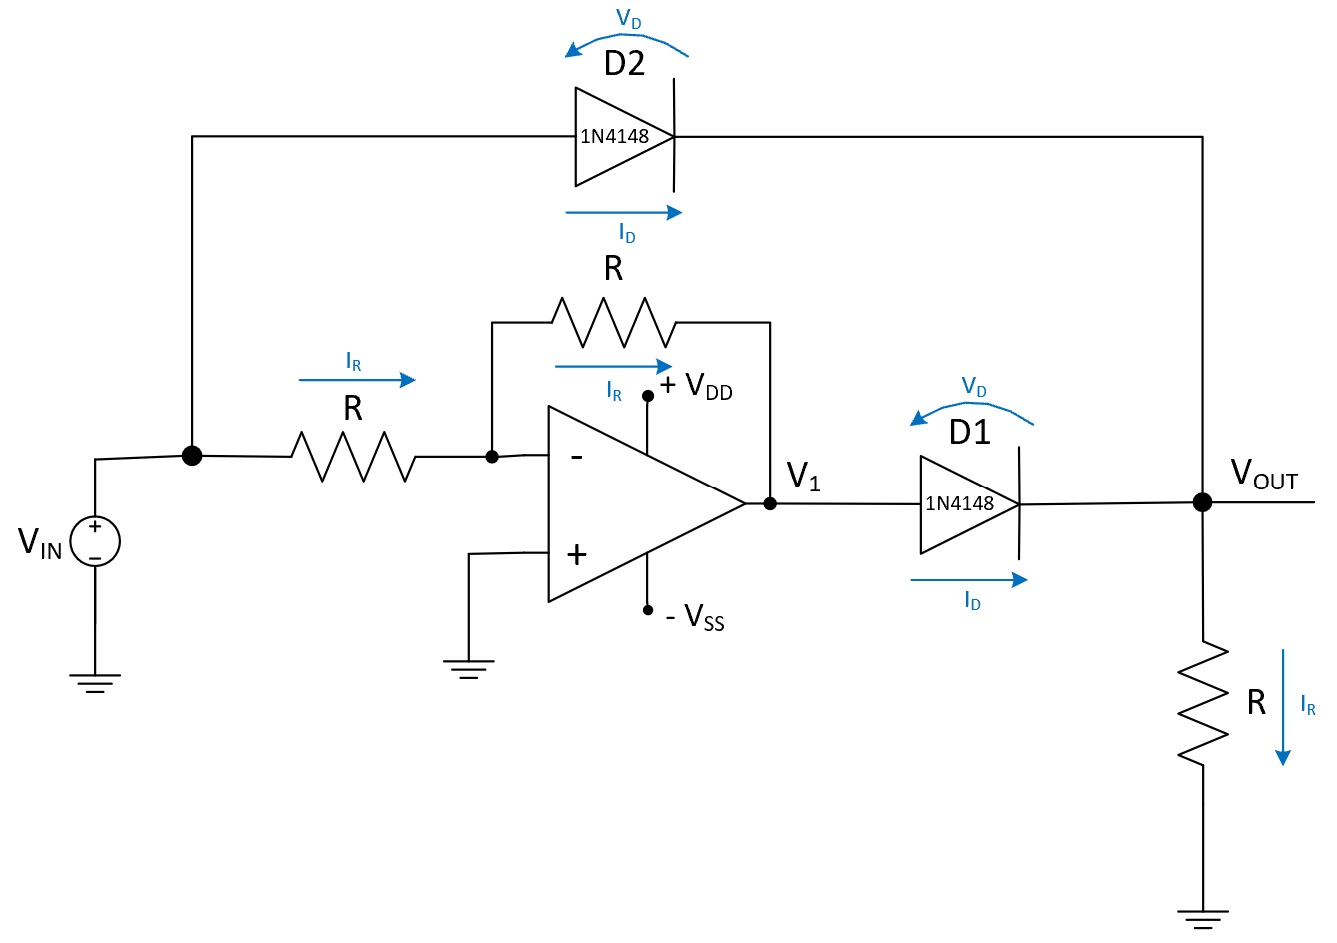
\includegraphics[height=7cm]{immagini/schema3}
	\caption{Schema del raddrizzatore a doppia semionda.}
	\label{figura:schema3}
\end{figure}
In aggiunta l'amplificatore si trova in configurazione invertente e per la presenza di resistenze con valori equivalenti presenta un guadagno pari a -1. Di fatto si comporta come un buffer invertente e questo lo si può notare dalla figura \ref{figura:TEK00023} in cui sono mostrati i segnali $\displaystyle\mathrm{V_{in}}$ e $\displaystyle\mathrm{V_{1}}$.
\begin{figure}[h]
	\centering
	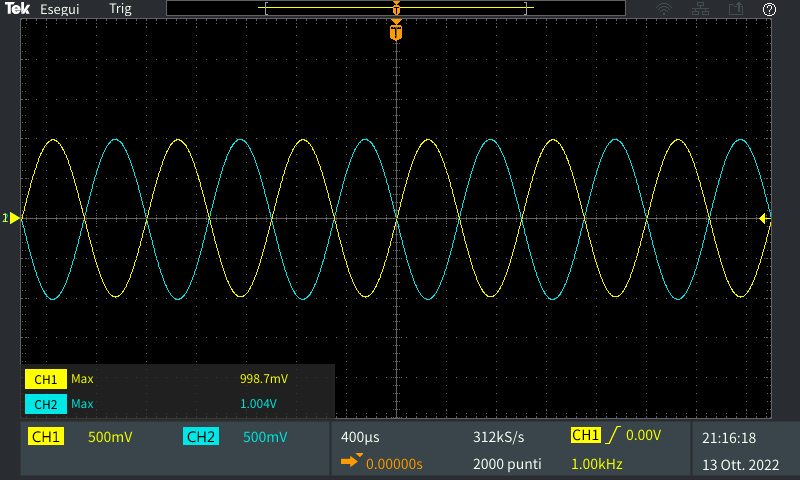
\includegraphics[height=6.5cm]{immagini/TEK00023}
	\caption{Comportamento di un buffer invertente.}
	\label{figura:TEK00023}
\end{figure}
\\La funzione di trasferimento corrispondente a questo circuito è:

\begin{equation}
   \begin{cases}
   V_{in}\le \SI{-0.7}{\volt}\;\;\indent\indent\rightarrow \mathrm{D_1\; ON, D_2\;OFF}\;\; \Rightarrow V_{out} = -V_{in}-\SI{0.7}{\volt}\\
  \SI{-0.7}{\volt} < V_{in}< \SI{0.7}{\volt}\rightarrow \mathrm{D_1\; OFF, D_2\;OFF} \Rightarrow V_{out} = \SI{0}{\volt}\\
   V_{in}\ge \SI{0.7}{\volt}\;\;\;\;\;\indent\indent\rightarrow \mathrm{D_1\; OFF, D_2\;ON}\;\; \Rightarrow V_{out} = V_{in}-\SI{0.7}{\volt}
   \end{cases}
\end{equation}

\subsection{Analisi e dati sperimentali}
Come primo passo per la costruzione del circuito, sono stati misurati i valori dei componenti che verranno utilizzati. In particolare abbiamo scelto tre resistenze da \SI{12}{k\ohm}. Le loro misure sono state riportate nella tabella \ref{table:mis_res3}.
\begin{table}[h!]
	\centering
	\begin{tabular}{|c|c|c|}
		\cline{2-3} 
		\multicolumn{1}{c|}{} & \textbf{Valore nominale} & \textbf{Valore misurato}\\ 
		\hline
		$\mathbf{R_1}$ & \SI{12}{k\ohm} & \SI{11.802}{k\ohm} \\ 
		\hline
		$\mathbf{R_2}$ & \SI{12}{k\ohm} & \SI{11.947}{k\ohm} \\ 
		\hline
		$\mathbf{R_3}$ & \SI{12}{k\ohm} & \SI{11.885}{k\ohm} \\ 
		\hline
	\end{tabular}
	\caption{Misure delle resistenze utilizzate per il circuito.}
	\label{table:mis_res3}
\end{table}
\begin{figure}[h!]
	\centering
	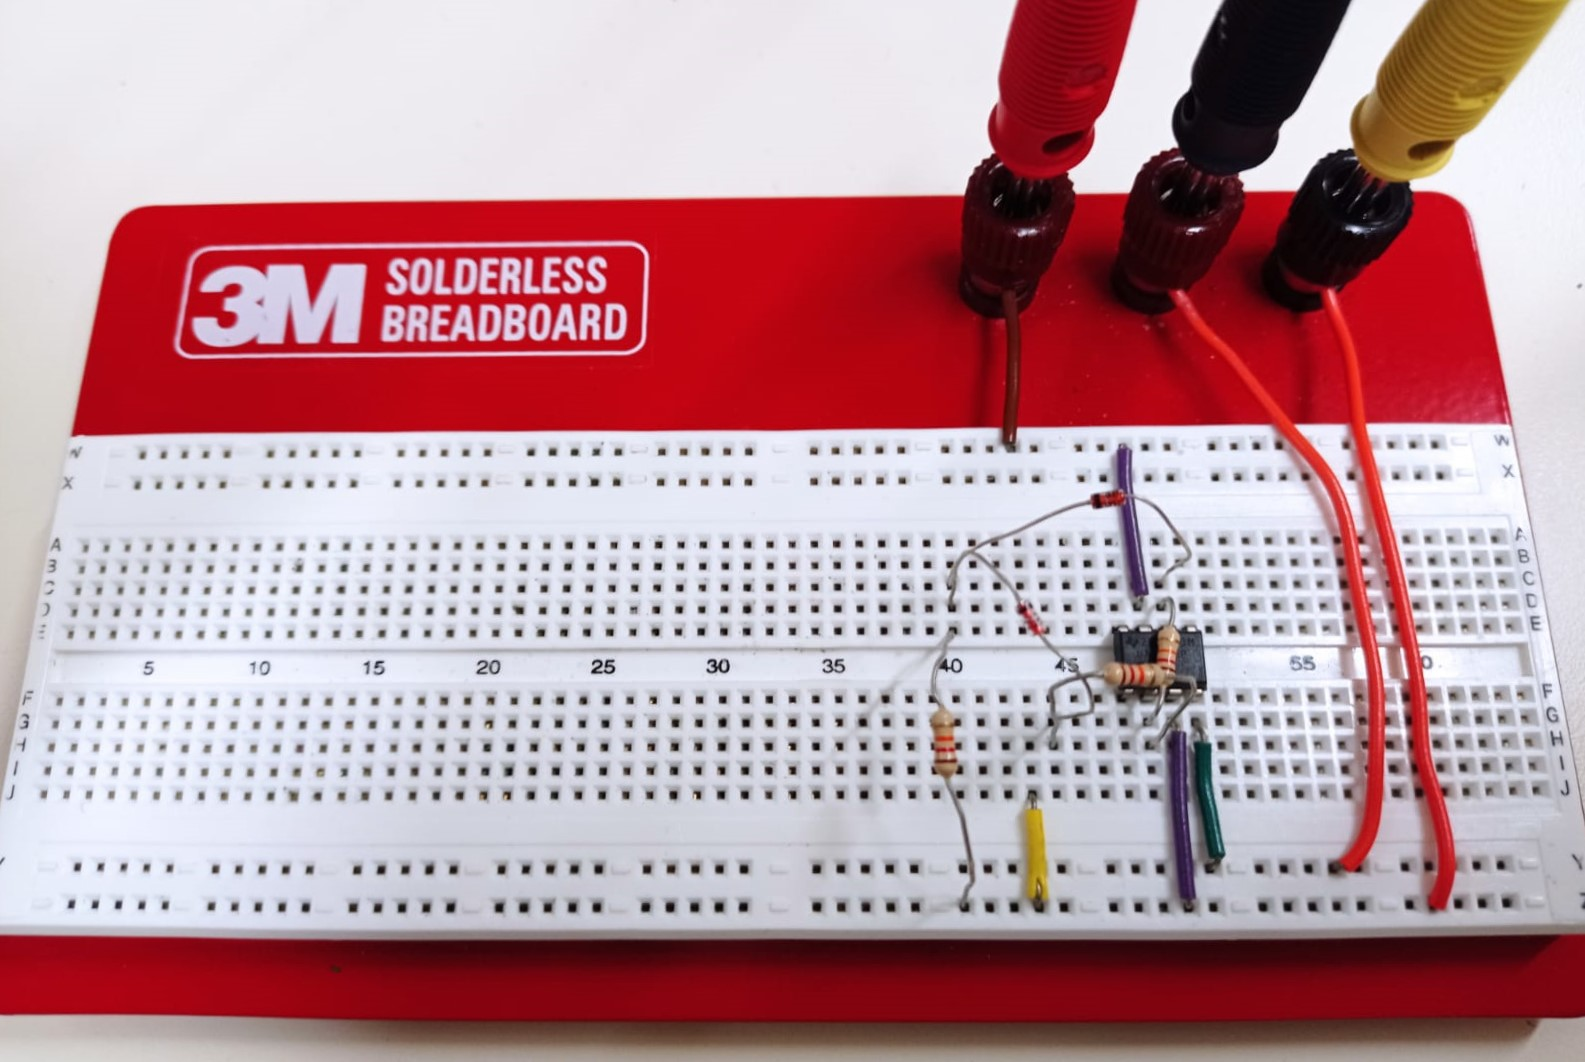
\includegraphics[height=7cm]{immagini/circuito3}
	\caption{Fotografia del raddrizzatore a doppia semionda realizzato in laboratorio.}
	\label{figura:circuito3}
\end{figure}
\\Una volta realizzato il circuito sulla breadboard, di cui si riporta la fotografia in figura \ref{figura:circuito3}, sono state effettuate delle misure (presenti nella tabella \ref{table:misure3}) dei valori di tensione nei vari nodi del circuito considerando i segnali in ingresso e in uscita a diverse frequenze (\SI{1}{k\hertz}, \SI{10}{k\hertz}, \SI{100}{k\hertz} e \SI{400}{k\hertz}). La forma d'onda utilizzata è sempre una sinusoide con un'ampiezza picco-picco pari a \SI{2}{\volt}.
\begin{table}[h!]
	\centering
	\begin{tabular}{|c|c|c|c|}
		\hline
		\textbf{Frequenza} & \boldmath$\displaystyle\mathrm{V_{PP,in}}$\textbf{ [V]} & \boldmath$\displaystyle\mathrm{{V_{PP,out}}}$\textbf{ [V]} & \boldmath$\Delta$\textbf{V [V]}\\
		\hline
		1 kHz & 0.980 & 0.520 & 0.460\\
		\hline
		10 kHz & 0.960 & 0.520 & 0.440\\
		\hline
		100 kHz & 0.980 & 0.520 & 0.460\\
		\hline
		400 kHz & 0.528 & 0.288 & 0.240\\
		\hline\end{tabular}
	\caption{Grandezze misurate ad ogni frequenza.}
	\label{table:misure3}
\end{table}
\\Per quanto riguarda la frequenza di \SI{1}{k\hertz}, come si può notare dalla figura \ref{figura:TEK00022}, i segnali presentano un andamento quasi ideale. A questa frequenza si può anche notare la presenza di un offset tra la tensione in ingresso e quella in uscita, che risulta pari a \SI{0.460}{\volt}.
\begin{figure}[h!]
	\centering
	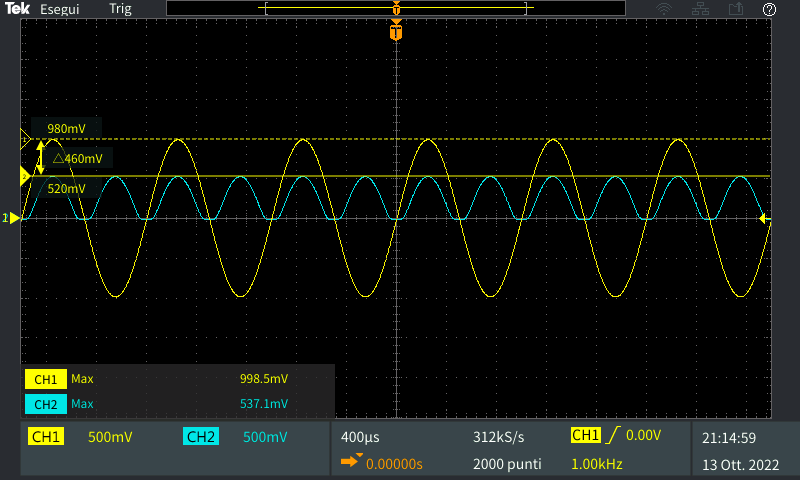
\includegraphics[height=6cm]{immagini/TEK00022}
	\caption{Segnali di $\mathrm{V_1}$ e di $\mathrm{V_{out}}$ con frequenza di \SI{1}{k\hertz}.}
	\label{figura:TEK00022}
\end{figure}
\\Invece se ad esempio si considera la frequenza di \SI{100}{k\hertz}, come si può notare dalla figura \ref{figura:TEK00025}, si vede che i segnali presentano una curva più estesa nella fase di spegnimento del diodo rispetto a quella della fase di accensione del diodo stesso. Questo andamento risulta ancora più accentuato nella figura \ref{figura:TEK00030} in cui la frequenza considerata è di \SI{400}{k\hertz}. Questa distorsione è causata dallo spegnimento dei diodi, perché il tempo di spegnimento è più lungo del periodo del circuito e questo causa un ritardo nella forma d'onda. A questa frequenza vediamo anche che scompaiono le semionde negative, perché non vengono più raddrizzate, sempre per effetto del ritardo.
\begin{figure}[h!]
	\centering
	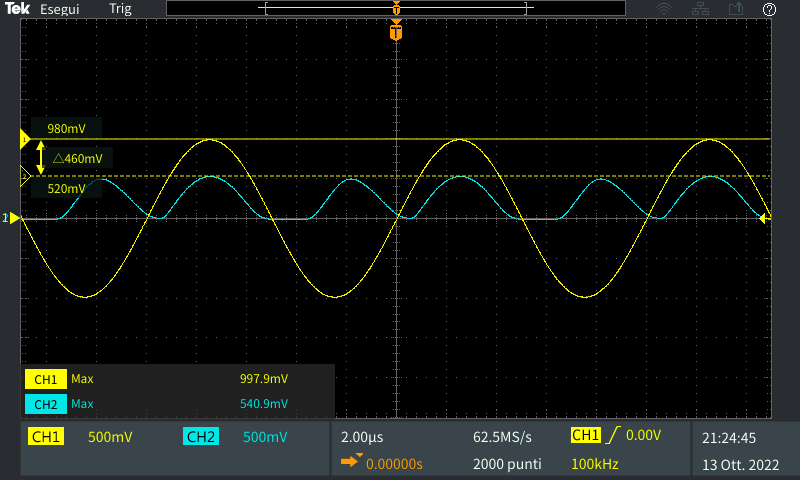
\includegraphics[height=6cm]{immagini/TEK00025}
	\caption{Segnali di $\mathrm{V_1}$ e di $\mathrm{V_{out}}$ con frequenza di \SI{100}{k\hertz}.}
	\label{figura:TEK00025}
\end{figure} 
\begin{figure}[h!]
	\centering
	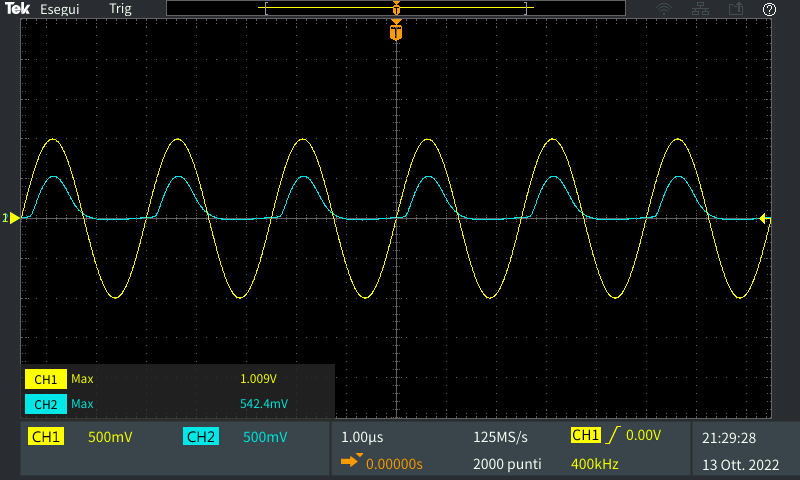
\includegraphics[height=6cm]{immagini/TEK00030}
	\caption{Segnali di $\mathrm{V_1}$ e di $\mathrm{V_{out}}$ con frequenza di \SI{400}{k\hertz}.}
	\label{figura:TEK00030}
\end{figure} 
\\Per frequenze maggiori, non ha senso studiare il circuito perché sappiamo che la banda di funzionamento del nostro OPAMP è limitata a circa \SI{100}{k\hertz} e anche la velocità di risposta dei diodi è stata superata.\par
Come si può notare dai grafici di questo circuito, il raddrizzatore a doppia semionda risolve il problema causato dallo swing della tensione $\displaystyle\mathrm{V_1}$ del secondo raddrizzatore analizzato. In questo modo la tensione in uscita all'OPAMP evita di raggiungere i valori delle alimentazioni dell'amplificatore stesso e di determinare proprio degli swing in tensione, che hanno l'effetto di rendere il circuito più lento.\par 
Permane però la caduta di tensione data dalla giunzione p-n dei diodi, perciò il segnale in uscita è leggermente attenuato. Questo può essere critico se il segnale da raddrizzare ha una piccola ampiezza.

%----------------------------------------------------------------------------------------

\end{document}
